\section{Matched-initial-state fluid comparisons}
\label{sec:controls}
\subsection{Intervention and implementation}
The initial-state discrepancy motivates an initialization sensitivity
experiment with both fluid models. The four cases use the posted one- and
two-fluid initializers and aggregate-PIC-matched versions of each. The
four-case intervention, solver settings and primary endpoint measurements
were pinned before evolution. The matched state contains the
archived PIC density, three ordinary-velocity momentum densities and six
uncentered second moments at every cell. No smoothing, pressure repair or
fitted drift correction is applied. The original electromagnetic fields,
domain, $480\times640$ grid, periodic boundaries, time stepper, CFL, closures
and source terms are retained.

For two fluids the original smooth positive weights $w_s(y)$ multiply the
entire aggregate conserved vector. With $w_1+w_2=1$ and
$0.03\leq w_s\leq0.97$, this preserves the aggregate state and gives common
velocity and population pressures $P_s=w_s P$. It matches aggregate moments
through second order, rather than the PIC's sharp tags, full distributions
or intrinsic third moments. The intervention also imports sampled spatial
variation. Its later effect cannot be attributed to the current mismatch,
proper-momentum convention or thermal spread alone.

The tested Gkeyll implementation is built from clean source commit
\href{https://github.com/liangwang0734/gkyl/tree/9663ea594e80f68eb305378e14512db390440e6b}{\texttt{9663ea594e80}}.
All 1,998 native and Lua source files are unchanged; the source archive,
compiler/dependency locks, installed runtime and executable hashes are
recorded. The archived identifier \texttt{9663ea594e80+} does not identify
its local changes or a unique executable. The clean baseline is therefore
compared with the saved source-fluid state before interpreting the matched
comparison. A compatibility failure with an older 2020 binary was retained;
that binary supplies none of the new evolution results.

Native initial-output tests reproduce the original arrays bit-for-bit.
The matched one-fluid conserved vector agrees bit-for-bit with its target.
Both matched two-fluid splits agree bit-for-bit with their weighted targets;
their aggregate differs by at most $1.11\times10^{-16}$, with pressure error
at most $4.16\times10^{-17}$. All eight stored field components are unchanged.
Every tested initial fluid population and aggregate PIC target passes positive-density and
positive-definite covariance-pressure checks. These conformance tests do
not establish identity with the historical dirty build.

Each case preserves \texttt{tEnd=600}, \texttt{nFrame=60} and the original
$4\times4$ MPI decomposition. Gkeyll's output trigger acts after accepted
steps, without forcing an exact output time. A native stop request is issued
only after the regular frame-30 files are closed, stable and consistent in
their stored metadata; their hashes are checked again after process exit.
Subsequent frames are excluded. Native rank logs and console output are
also checked for the fatal timestep-collapse marker, including when a
numerical failure returns exit code zero. An absent or failed case cannot
supply a paired measurement. Three cases reach guarded regular frame~30.
The matched two-fluid run instead exits with code~1 after an assertion in
\texttt{MomentSpecies.lua:495}, without a native stop request or regular
frame~30. Its last closed regular output is frame~22 at
$t=220.00011000001655\,\omega_{pe}^{-1}$. That is a saved-output time, not
the exact assertion time. The logged transient does not establish the
failing cell, population or numerical cause. No final comparison or full
saved-history pressure audit is inferred for this failed run.

\subsection{Comparison quantities and scope}
Unit electron mass and charge $-1$ give $J_z=-\rho u_z$. We recover aggregate
pressure after summing the conserved population vectors. Current, density,
$P_{xx}$ and $P_{zz}$ errors use every one of the 307,200 cells. Relative
$\ell^2$ error is $\norm{A-A_{\rm PIC}}_2/\norm{A_{\rm PIC}}_2$; a zero
reference norm gives an explicit null value, rather than an added small
denominator. Separately reported profile norms first average over $x$ and
can cancel transverse structure. They are not full-grid error norms.
This is physical moment current, rather than the unavailable native
deposited PIC current.

For two populations the reconstructable population-recentering contribution is
\[
q^{\rm CS}_{xxx}=\sum_s\left[3P_{s,xx}(u_{s,x}-u_x)
                 +\rho_s(u_{s,x}-u_x)^3\right].
\]
Its primary PIC comparator uses the deposited tag populations and documented
first and second moments. This contribution depends on the decomposition.
The finite local-isotropization model supplies a divergence, so it does not
uniquely specify the complete intrinsic population heat-flux tensors. In
particular, a one-fluid recentering contribution is zero by definition and
does not imply zero full heat transport.

A separate central PIC $q_{xxx}$ reconstruction is conditional on treating
the posted third-product diagnostics as unnormalized raw moments. The
deposit explicitly defines its first/second diagnostics, but the third-product
names and units do not verify that normalization. Algebraic reconstruction
checks and this assumption are recorded separately. The four ordinary-moment
comparisons and tagged-$q^{\rm CS}$ comparison do not depend on it.
Exact-vacuum PIC tags contribute zero without a density floor. Their small
negative diagnostic covariance eigenvalues, down to approximately
$-3.84\times10^{-11}$ and $-2.25\times10^{-11}$, are retained explicitly;
the tag contribution is an algebraic diagnostic rather than certification
of strictly positive-definite population states.

The PIC reference has stored time $300.0015\,\omega_{pe}^{-1}$ and iteration
4500. Source-fluid frame-30 times are $300.0001500000136$ and
$300.0499847996274$. New output times are likewise read from the files.
Raw-frame comparisons use these actual times without interpolation. A
matched frame number is not an exactly common physical time.

\subsection{Realizability is stronger than positive coordinate pressures}
For any nonnegative population distribution and any real vector $\bm a$,
\[
 \bm a^{\mathsf T}P_s\bm a
 =m_s\int f_s\,[\bm a\!\cdot(\bm v-\bm u_s)]^2\,\dd^3v\ge0.
\]
Consequently, covariance pressure must be positive semidefinite. Positive
coordinate diagonals test only three directions; they do not impose this
condition for every direction. The thermal-fluid comparison guard additionally
requires strict positive definiteness.

The clean source's
\href{https://github.com/liangwang0734/gkyl/blob/9663ea594e80f68eb305378e14512db390440e6b/Eq/TenMoment.lua}{\texttt{TenMoment:isPositive}}
in lines 128--136 checks density and the three recovered diagonal pressures
for NaNs and negative values. It does not inspect off-diagonal components,
principal minors or eigenvalues.
\href{https://github.com/liangwang0734/gkyl/blob/9663ea594e80f68eb305378e14512db390440e6b/App/Species/MomentSpecies.lua}{\texttt{MomentSpecies:checkInv}}
applies that predicate cellwise and combines it across MPI ranks.
The code's primitive conversion independently confirms the off-diagonal
packing, without an engineering factor of two.

The clean unmatched two-fluid endpoint gives a concrete witness. Population~1
has 16 indefinite cells, with
$\min\lambda(P_1)/(m_en_0c^2)=-0.0014125968$. At the raw
cell center $(x/d_e,y/d_e)=(8.45,-18.35)$ its rounded covariance is
\[
\frac{P_1}{m_en_0c^2}=10^{-3}
\begin{pmatrix}
 3.0547143&-2.1601719&-3.1063763\\
 -2.1601719&6.1297082&-0.5752234\\
 -3.1063763&-0.5752234&1.4115557
\end{pmatrix}.
\]
Density and all three diagonals are positive, but the unrounded dimensionless
tensor's $xz$ principal minor is approximately $-5.33767422\times10^{-6}$ and its determinant is
$-4.80357889\times10^{-8}$. Independent long-double centering and quadratic
form/minor checks corroborate the eigenvalue result. Population~2 and the
aggregate remain positive definite. Aggregate positivity does not make an
unrealizable component distribution admissible, so primary error metrics for
this endpoint are withheld rather than computed after clipping or masking.

The corresponding original archived endpoint is positive definite in every
cell of both populations and their aggregate. Its time is later by
$0.0061523168\,\omega_{pe}^{-1}$. The witness therefore establishes a failure
of the identified clean reconstruction, not of the unavailable dirty build.
The diagonal predicate makes normal native completion consistent with the
failure; it does not identify the first loss time or the split operator that
produced it.

Checking only initial and final states is also insufficient. The full
saved-history audit was added after the clean two-fluid endpoint failed the
strict collector; it is an additional diagnostic, not a prespecified primary
performance measurement. A hash-bound
scan of all regular saved frames 0--30 finds that the unmatched one-fluid
case has 9, 18 and 7 indefinite cells at saved times near 220, 230 and 240,
despite positive-definite endpoints. The matched one-fluid case has 5, 23,
47, 30 and 5 at saved times near 220--260. Their most negative eigenvalues
are $-0.0017235454$ and $-0.0053207379$ in units of $m_en_0c^2$,
respectively. The two-fluid unmatched
population~1 also fails at saved frames 19 and 22, with two cells each,
in addition to its rejected endpoint; its population~2 and aggregate pass
all 31 saved checks. These are observed saved snapshots, not every accepted
timestep or proof of the first physical-time failure. The Gaussian entropy
diagnostic in Section~\ref{sec:entropy} is restricted to positive-definite
states and is not applied to the indefinite tensors.

\begin{table}[tbp]
\centering\small
\caption{Native outcomes and saved-state admissibility. Endpoint eligibility uses the unchanged initial/final covariance checks. Eigenvalues are in units of $m_en_0c^2$. For successful runs, non-PSD counts are population--snapshot instances out of $31N_s$, not distinct spatial cells or every accepted timestep. The failed run has no regular-frame-30 endpoint or full-history audit; its missing entries are not zero failures. A numerical endpoint contrast does not validate a physical trajectory.}
\label{tab:control-outcomes}
\begin{tabular}{lrrrr}
\toprule
Case & Actual $t$ & Endpoint & Non-PSD samples & Minimum $\lambda(P_s)$ \\
\midrule
Unmatched, one & 300.000150 & eligible & 3/31 & $-0.00172355$ \\
Unmatched, two & 300.043832 & rejected & 3/62 & $-0.0014126$ \\
Matched, one & 300.000150 & eligible & 5/31 & $-0.00532074$ \\
Matched, two & --- & no frame 30 & --- & --- \\
\bottomrule
\end{tabular}
\end{table}


\begin{figure}[tbp]
\centering
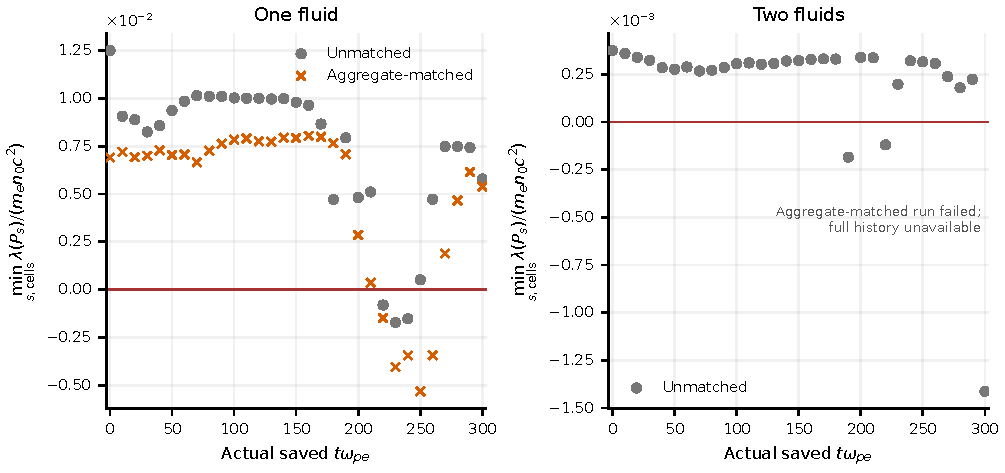
\includegraphics[width=\linewidth]{../figures/numerical-endpoints-pressure-history.pdf}
\caption{Smallest population covariance eigenvalue over all cells at each
actual regular saved time for successfully completed runs. The failed matched
two-fluid history is explicitly unavailable. Each point is a separate spatial minimum, not a
tracked fluid parcel. The aggregate is not substituted for the population
test. Negative points are non-realizable covariances. No connecting lines or
interpolation are used, and unobserved timesteps are not certified by positive
saved points. These are clean-source numerical cases, not the original
archived trajectories.}
\label{fig:pressure-realizability}
\end{figure}

\subsection{Numerical endpoint sensitivity and baseline fidelity}
The one-fluid unmatched and matched endpoints both pass the strict state
checks and occur at exactly $t=300.0001500000136\,\omega_{pe}^{-1}$. Relative
complete-grid $\ell^2$ errors against the same PIC reference change from
$3.9763\%$ to $3.4774\%$ in density, $28.3046\%$ to $26.5123\%$ in $J_z$,
$36.2872\%$ to $28.8547\%$ in $P_{xx}$ and $34.6557\%$ to $30.7718\%$ in
$P_{zz}$. The changes are approximately $-0.4990$, $-1.7923$, $-7.4324$ and
$-3.8840$ percentage points. They quantify the numerical endpoint response
to the full aggregate-moment intervention; they are not current-only effects
or validation of physical dynamics.

The clean one-fluid baseline differs from its archived source counterpart
by $0.2104\%$, $0.7143\%$, $0.7158\%$ and $1.2758\%$ in the same respective
field norms, at identical times. The maximum absolute density discrepancy is
$0.09399n_0$, so small global norms must not be read as uniform pointwise
bounds. The exact original dirty implementation is not recovered. The
two-fluid baseline's population failure prevents a validated same-runtime
two-fluid initialization pair; no such effect is inferred from a positive
aggregate or from comparison with a different archived executable.

\begin{table}[tbp]
\centering\small
\caption{Clean unmatched versus archived source-fluid output at eligible endpoints. Relative complete-grid $\ell^2$ differences are percentages, with the archived state as denominator. The final column is the combined norm of all eight stored field components, not an electromagnetic energy error. $\Delta t$ is the actual clean-minus-archived time. These norms are neither uniform pointwise bounds nor trajectory-admissibility certificates.}
\label{tab:baseline-fidelity}
\begin{tabular}{lrrrrrr}
\toprule
Fluids & $\Delta t$ & $n$ & $J_z$ & $P_{xx}$ & $P_{zz}$ & Stored fields \\
\midrule
One & 0 & 0.2104 & 0.7143 & 0.7158 & 1.2758 & 0.0695 \\
\bottomrule
\end{tabular}
\end{table}

\begin{table}[tbp]
\centering\small
\caption{Numerical endpoint complete-grid relative $\ell^2$ errors (percent) against the archived PIC snapshot at $t=300.0015$. Every actual fluid output time is retained; no temporal interpolation is applied. Endpoint agreement does not validate a physical trajectory. Withheld entries are not zero errors.}
\label{tab:control-errors}
\begin{tabular}{lrrrrr}
\toprule
Case & Actual $t$ & $n$ & $J_z$ & $P_{xx}$ & $P_{zz}$ \\
\midrule
Archived source, one & 300.000150 & 3.973 & 28.340 & 36.357 & 34.577 \\
Archived source, two & 300.049985 & 2.648 & 21.736 & 34.261 & 31.522 \\
Clean baseline, one & 300.000150 & 3.976 & 28.305 & 36.287 & 34.656 \\
Clean baseline, two (withheld) & 300.043832 & --- & --- & --- & --- \\
Matched, one & 300.000150 & 3.477 & 26.512 & 28.855 & 30.772 \\
Matched, two (withheld) & --- & --- & --- & --- & --- \\
\bottomrule
\end{tabular}
\end{table}


\begin{figure}[tbp]
\centering
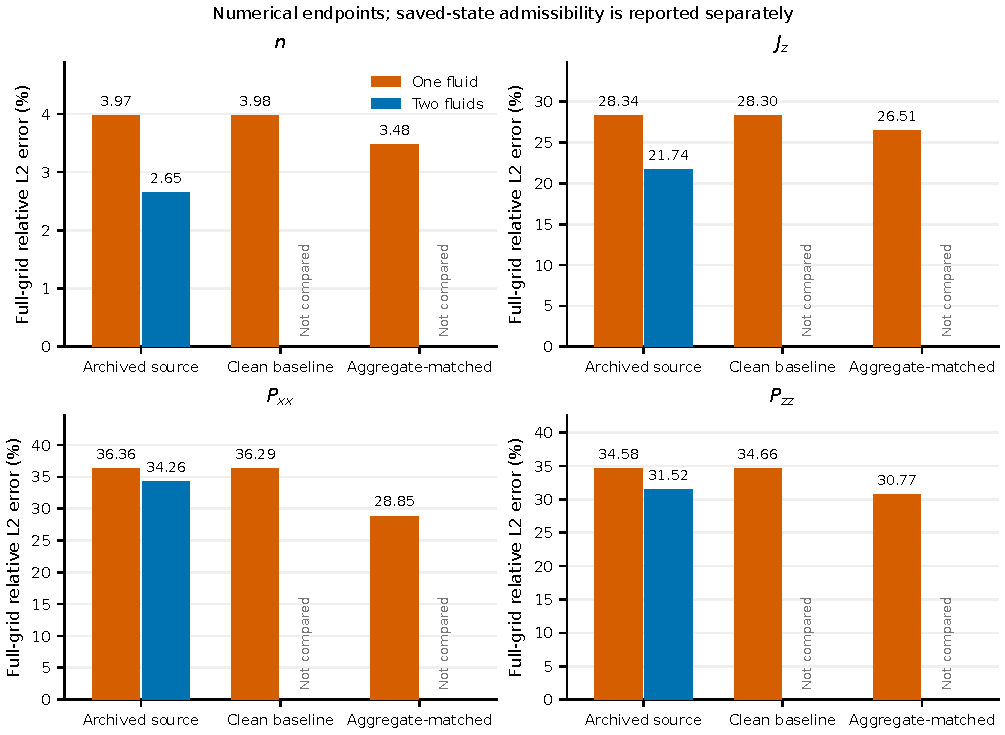
\includegraphics[width=\linewidth]{../figures/numerical-endpoints-errors.pdf}
\caption{Complete-grid numerical endpoint errors against the same archived
PIC reference. Withheld, nonconforming endpoints have no error bar; the
annotation is not a zero error. Source archives supply context, while the
same-runtime one-fluid pair isolates the specified initialization intervention
at identical endpoint times. Its non-realizable saved histories preclude a
physical-trajectory validation claim.}
\label{fig:numerical-endpoint-errors}
\end{figure}

\begin{figure}[tbp]
\centering
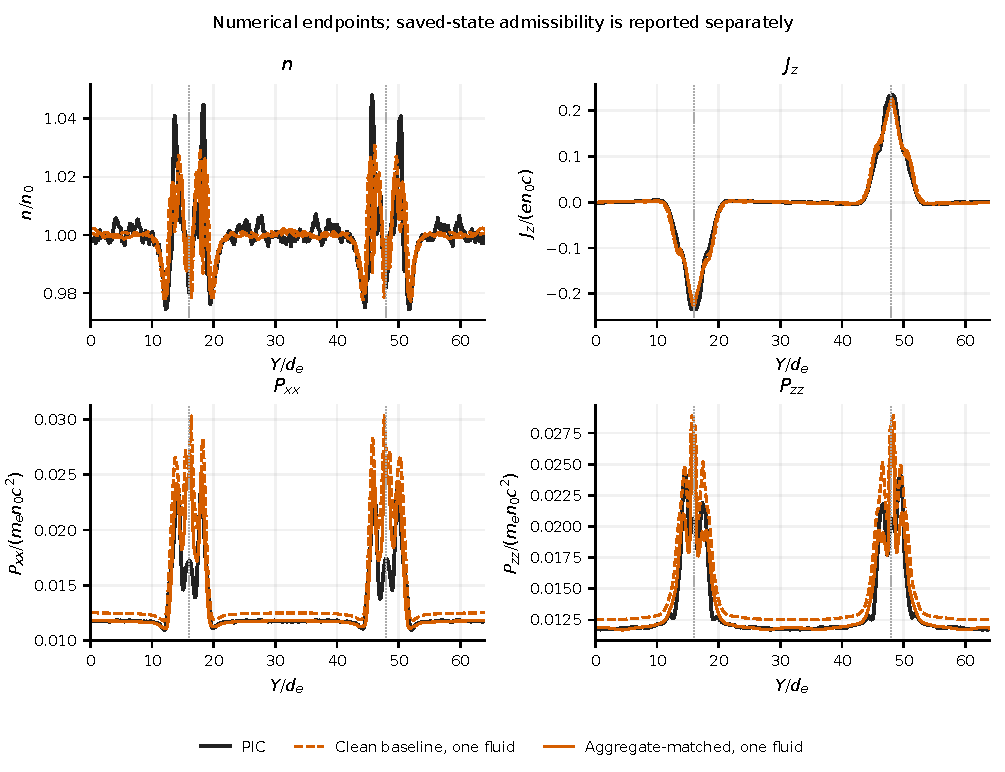
\includegraphics[width=\linewidth]{../figures/numerical-endpoints-profiles.pdf}
\caption{Full-domain, $x$-averaged numerical endpoint profiles for eligible
clean baseline and aggregate-matched cases, with the PIC reference. Missing
curves are withheld cases, not vanishing fields. The projected profiles are
distinct from the complete-grid norms in Figure~\ref{fig:numerical-endpoint-errors}.
Positive endpoint covariances do not erase the saved intermediate failures.}
\label{fig:numerical-endpoint-profiles}
\end{figure}

The four terminal native outcomes, endpoint metric eligibility and
saved-snapshot diagnoses remain separate in the accompanying machine-readable
record: three normal native completions, one failed execution, three full
saved-history scans and two eligible control endpoints. The failed run is
not counted as a completed comparison or a 31-snapshot scan.
No rejected endpoint receives primary performance metrics. The strict
full-set comparison gate remains false when an endpoint is rejected; the
explicit subset route reports numerical endpoints with their history failures.
The~experiment uses one grid, one closure setting and one sampled initial
target. There is no ensemble, resolution-convergence result, exact original
executable recovery or physical causal bound. Lower endpoint errors and more
saved covariance failures can coexist, as the one-fluid contrast demonstrates.
